% Этот шаблон документа разработан в 2014 году
% Данилом Фёдоровых (danil@fedorovykh.ru) 
% для использования в курсе 
% <<Документы и презентации в \LaTeX>>, записанном НИУ ВШЭ
% для Coursera.org: http://coursera.org/course/latex .
% Исходная версия шаблона --- 
% https://www.writelatex.com/coursera/latex/5.1

\documentclass[t]{beamer}  % [t], [c], или [b] --- вертикальное выравнивание на слайдах (верх, центр, низ)
%\documentclass[handout]{beamer} % Раздаточный материал (на слайдах всё сразу)
%\documentclass[aspectratio=169]{beamer} % Соотношение сторон

%\usetheme{Berkeley} % Тема оформления
%\usetheme{Bergen}
%\usetheme{Szeged}

%\usecolortheme{beaver} % Цветовая схема
%\useinnertheme{circles}
%\useinnertheme{rectangles}

\usetheme{HSE}

%%% Работа с русским языком
\usepackage{cmap}					% поиск в PDF
\usepackage{mathtext} 				% русские буквы в формулах
\usepackage[T2A]{fontenc}			% кодировка
\usepackage[utf8]{inputenc}			% кодировка исходного текста
\usepackage[english,russian]{babel}	% локализация и переносы
\usepackage{minted}					% листинги кода

%% Beamer по-русски
\newtheorem{rtheorem}{Теорема}
\newtheorem{rproof}{Доказательство}
\newtheorem{rexample}{Пример}

\newcommand\pro{\item[$+$]} 		% плюс в списке
\newcommand\con{\item[$-$]} 		% минус в списке


\newcommand{\questionframe}[2]{
    \frame[c,plain]{
        \centering\huge
        \textbf{\structure{#1}}
        \par\bigskip
        #2
    }
}

%%% Дополнительная работа с математикой
\usepackage{amsmath,amsfonts,amssymb,amsthm,mathtools} % AMS
\usepackage{icomma} % "Умная" запятая: $0,2$ --- число, $0, 2$ --- перечисление

%% Номера формул
%\mathtoolsset{showonlyrefs=true} % Показывать номера только у тех формул, на которые есть \eqref{} в тексте.
%\usepackage{leqno} % Нумерация формул слева

%% Свои команды
\DeclareMathOperator{\sgn}{\mathop{sgn}}

%% Перенос знаков в формулах (по Львовскому)
\newcommand*{\hm}[1]{#1\nobreak\discretionary{}
{\hbox{$\mathsurround=0pt #1$}}{}}

%%% Работа с картинками
\usepackage{graphicx}  % Для вставки рисунков
\graphicspath{{images/}{images2/}}  % папки с картинками
\setlength\fboxsep{3pt} % Отступ рамки \fbox{} от рисунка
\setlength\fboxrule{1pt} % Толщина линий рамки \fbox{}
\usepackage{wrapfig} % Обтекание рисунков текстом

%%% Работа с таблицами
\usepackage{array,tabularx,tabulary,booktabs} % Дополнительная работа с таблицами
\usepackage{longtable}  % Длинные таблицы
\usepackage{multirow} % Слияние строк в таблице

%%% Программирование
\usepackage{etoolbox} % логические операторы

%%% Другие пакеты
\usepackage{lastpage} % Узнать, сколько всего страниц в документе.
\usepackage{soul} % Модификаторы начертания
\usepackage{csquotes} % Еще инструменты для ссылок
%\usepackage[style=authoryear,maxcitenames=2,backend=biber,sorting=nty]{biblatex}
\usepackage{multicol} % Несколько колонок

%%% Картинки
\usepackage{tikz} % Работа с графикой
\usepackage{pgfplots}
\usepackage{pgfplotstable}

\title{Поддержка типа dynamic в JVM}
%\subtitle{}
\author{Алексей Степанов}
\date{\today}
\institute[СПб АУ НОЦНТ РАН]{Научный руководитель:  Андрей Бреслав \\
    \vspace{0.7cm}
    САНКТ-ПЕТЕРБУРГСКИЙ АКАДЕМИЧЕСКИЙ УНИВЕРСИТЕТ \\
    \vspace{0.7cm}
}

\begin{document}

\frame[plain]{\titlepage}	% Титульный слайд

\section{Введение}
 
\begin{frame}
	\frametitle{\insertsection} 
    Типизация в языках программирования
	\begin{itemize}
    	\item Статическая типизация
       	\item Динамическая типизация
        \item Постепенная типизация
	\end{itemize}    
\end{frame}

\begin{frame}
	\frametitle{\insertsection} 
	\begin{block}{Постепенная типизация}
		Постепенная типизация - система типов, в которой часть переменных и выражений может быть типизированна, и их корректность 					проверяется в момент компиляции, а часть может быть не типизированна, и об ошибках в них мы узнаем во время исполнения.
	\end{block}

	\begin{block}{Преимущества}
		\begin{itemize}
	    	\item eval
	        \item DSL (Gradle)
   	       	\item DOM
		\end{itemize}    
    \end{block}
\end{frame}

\subsection{DOM}

\begin{frame}[fragile]
	\frametitle{\insertsection} 
    \framesubtitle{\insertsubsection}
	\begin{block}{Удобный доступ к полям и методам}
	\begin{minted}{csharp}
dynamic x = dom.html.body.tables.main.tr.td;
	\end{minted}
    \end{block}
    
    \begin{block}{Почему не Object?}
    \begin{minted}{csharp}
Scriptobj.SetProperty("Cnt",((int)GetProperty("Cnt"))+1);
scriptobj.Cnt += 1;
	\end{minted}
    \end{block}
\end{frame}


\subsection{Постепенная типизация}

\begin{frame}[fragile]
	\frametitle{\insertsection} 
    \framesubtitle{\insertsubsection}
	\begin{block}{Варианты постепенной типизации}
		\begin{table}
			\begin{tabular}{l | c  }
				От динамической типизации & От статической типизации \\
				\hline \hline
				Python & C\# \\ 
				JavaScript & Scala\\
				Groovy &  Kotlin?  
			\end{tabular}
		% \caption{Triathlon results}
		\end{table}
    \end{block}
\end{frame}


\subsection{Обзор языков с постепенной типизацией}

\begin{frame}[fragile]
	\frametitle{\insertsection} 
    \framesubtitle{\insertsubsection}
	\begin{block}{Python: Type Hints}
	\begin{minted}{python}
def greeting(name: str) -> str:
    return 'Hello ' + name
	\end{minted}
    \begin{minted}{python}
AnyStr = TypeVar('AnyStr', str, bytes)
def concat(x: AnyStr, y: AnyStr) -> AnyStr:
    return x + y
	\end{minted}
    \end{block}
\end{frame}



\begin{frame}[fragile]
	\frametitle{\insertsection} 
    \framesubtitle{\insertsubsection}
\begin{block}{JavaScript: Flow}
	\begin{minted}{javascript}
// @flow
function bar(x): string {
  return x.length;
}
bar('Hello, world!');
	\end{minted}
    \begin{alertblock}{Flow output}
    \begin{verbatim}
3:   return x.length; - number. This type is incompatible 
with the expected return type of
2: function bar(x): string { -string 
    \end{verbatim}
    \end{alertblock}
    \end{block}
\end{frame}


\begin{frame}[fragile]
	\frametitle{\insertsection} 
    \framesubtitle{\insertsubsection}
\begin{block}{Scala}
	\begin{minted}{scala}
class MyRouter extends Dynamic{
    def selectDynamic(name: String): T = {}
    def updateDynamic(name: String)(value: T): Unit = {}
    def applyDynamic(methodName: String)(args: Any*) {
       println(s"You called '$methodName' method with " +
          s"following arguments: ${args mkString ", "}")
     }
     def applyDynamicNamed(name: String)
     			(args: (String, Any)*) {
        println(s"You called '$name' method with " +
            s"following argiuments: 
            ${args map (a=>a._1+"="+a._2) mkString ","}")
    }
 }
	\end{minted}
\end{block}
\end{frame}

\begin{frame}[fragile]
	\frametitle{\insertsection} 
    \framesubtitle{\insertsubsection}
\begin{block}{Scala}
\begin{itemize}
        \pro Поддержка в ScalaJS
        \pro Возможность написать свою логику диспетчеризации
        \con Нет стандартных реализаций
        \con Своя логика будет скорее всего медленная
%        \item neutral
   \end{itemize}
\end{block}
\end{frame}


\begin{frame}[fragile]
	\frametitle{\insertsection} 
    \framesubtitle{\insertsubsection}
	\begin{block}{C\#}
		\begin{minted}{csharp}
dynamic obj = new MyObject();
obj.anyMethod(53);
		\end{minted}
	\end{block}
   	\begin{block}{Своё разрешение как в Scala}
		\begin{minted}{csharp}
public class MyDynamicImpl : DynamicObject{
   public override bool TryGetMember(
        GetMemberBinder binder, out object result){}
   public override bool TrySetMember(
        SetMemberBinder binder, object value){}
}
        \end{minted}
	\end{block}
\end{frame}

\begin{frame}[fragile]
	\frametitle{\insertsection} 
    \framesubtitle{\insertsubsection}
	\begin{block}{C\# ExpandoObject}
		\begin{minted}{csharp}
XElement contactXML =
    new XElement("Contact",
        new XElement("Name", "Patrick Hines"),
        new XElement("Phone", "206-555-0144"),
        new XElement("Address",
            new XElement("Street1", "123 Main St"),
            new XElement("City", "Mercer Island"),
            new XElement("State", "WA"),
            new XElement("Postal", "68042")
        )
    );
		\end{minted}
	\end{block}
\end{frame}


\begin{frame}[fragile]
	\frametitle{\insertsection} 
    \framesubtitle{\insertsubsection}
	\begin{block}{C\# ExpandoObject}
		\begin{minted}{csharp}
dynamic contact = new ExpandoObject();
contact.Name = "Patrick Hines";
contact.Phone = "206-555-0144";
contact.Address = new ExpandoObject();
contact.Address.Street = "123 Main St";
contact.Address.City = "Mercer Island";
contact.Address.State = "WA";
contact.Address.Postal = "8402";
		\end{minted}
	\end{block}
\end{frame}


\begin{frame}[fragile]
	\frametitle{\insertsection} 
  	\framesubtitle{\insertsubsection}
    \begin{block}{Dynamic Language Runtime}
		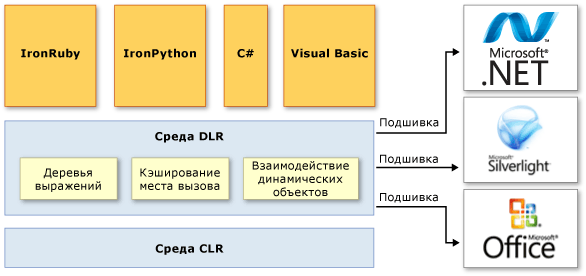
\includegraphics[height=0.55\paperheight]{dlr} 
    \end{block}
\end{frame}


\section{Вопросы постепенной типизации}
\begin{frame}
	\frametitle{\insertsection} 
    \begin{block}{Возникающие вопросы}
		\begin{itemize}
          \item Где хранить информацию о типе?
          \item Как хранить динамически типизированный объект?
          \item Как выбирать перегрузки при вызове методов?
          \item Как сделать всё оптимально и быстро?
		\end{itemize}
	\end{block}
\end{frame}

\subsection{Разрешение перегрузок}
\begin{frame}
	\frametitle{\insertsection} 
  	\framesubtitle{\insertsubsection}
	\begin{itemize}
       \item В динамических языках возможна перегрузка только по числу параметров
       \item В статически типизированных языках у нас доступна перегрузка по типам аргументам
    \end{itemize}
    \begin{block}{Возникающий вопрос}
		\begin{itemize}
          \item Можем ли мы при постепенной типизации делать во время исполнения всё то же что мы делали во время компиляции?
          \item<2> Ответ: Нет.
          		\begin{itemize}
                	\item Это дорого
                    \item Это невозможно
                \end{itemize}
%          \alt<4>{Это \alert{четвертый} слайд}{Это не четвертый слайд.}
		\end{itemize}
	\end{block}
\end{frame}

	
\begin{frame}
	\frametitle{\insertsection} 
  	\framesubtitle{\insertsubsection}
    \begin{block}{Groovy}
		\begin{enumerate}
			\item  Получить список всех методов с подходящим именем
			\item  Удалить все методы которые не подходят к данному вызову
			\item  Если осталось больше одного метода, то вычислить метрику на на методах
			\item  Метод с наименьшим значением метрики выигрывает
			\item  Если имеется несколько методов с наименьшей дистанцией, то выдать исключение
		\end{enumerate}
	\end{block}
\end{frame}


\begin{frame}[fragile]
	\frametitle{\insertsection} 
  	\framesubtitle{\insertsubsection}
    \begin{block}{Groovy}
		\begin{minted}{groovy}
static foo(Object o, Integer i) { "Integer won" }
static foo(String s, Object o) { "String won" }

assert foo("potato", new Integer(6)) =~ "Integer"
		\end{minted}
	\end{block}
	\begin{block}{Полученная дистанция}
    \begin{itemize}
	    \item $\rho(String, Object) + \rho(Integer, Integer) == 1 + 0 == 1$
	    \item $\rho(String, String) + \rho(Integer, Object) == 0 + 2 == 2$ (Integer $\rightarrow$ Number $\rightarrow$ Object)
	\end{itemize}
    \end{block}
\end{frame}

\begin{frame}[fragile]
	\frametitle{\insertsection} 
  	\framesubtitle{\insertsubsection}
    \begin{block}{@CompileStatic разрешает типы только для локальных переменных}
	    \begin{minted}{groovy}
def foo(Object x){1} 
def foo(String x){2} 
def create(){ return "" } 
 
@CompileStatic 
def bar() { 
   assert foo("") == 2 
   assert foo(new Object()) == 1 
   assert foo(create()) == 1 
} 
 
bar()
		\end{minted}
    \end{block}
\end{frame}

\begin{frame}[fragile]
	\frametitle{\insertsection} 
  	\framesubtitle{\insertsubsection}
    \begin{block}{C\#}
\begin{itemize}
\item Во время компиляции мы проверяем что во время исполнения может подойти хотя бы один метод
\item По алгоритму похожему на используемый во время компиляции определяем лучший метод
\item Разницу между Object и dynamic не разрешаем
\end{itemize}
    \end{block}
\end{frame}

\begin{frame}[fragile]
	\frametitle{\insertsection} 
  	\framesubtitle{\insertsubsection}
    \begin{block}{JSmall - динамические теги типа}
    	    \begin{minted}{groovy}
public void XMLWriter::write(int e) { y}
public void XMLWriter::write(Integer e) { y}
public void XMLWriter::write(XMLElement e) { y}
public void XMLWriter::write(StructuredXMLElement e) { y}
public void XMLWriter::write(Serializable e) { y}
w:='XMLWriter' asJavaClass new.
i:= 10 type: 'int'.
obj :='StructuredXMLElement' asJavaClass new
         type: 'java.io.Serializable'
w write: i.
w write: obj.
w write: (obj type: 'StructuredXMLElement').
w write: obj.
		\end{minted}
\begin{itemize}
\item ву
\end{itemize}
    \end{block}
\end{frame}

\begin{frame}[fragile]
	\frametitle{\insertsection} 
  	\framesubtitle{\insertsubsection}
    \begin{block}{JSmall - динамические теги типа}
\begin{itemize}
\item Мы можем помечать перменные тегами типа
\item Тег типа используется только для разрешения вызовов, и никак не связан с реальным типом перменной
\item Все значения полученные из Java автоматически маркируются тегом типа
\end{itemize}
    \end{block}
\end{frame}

\begin{frame}[fragile]
	\frametitle{\insertsection} 
  	\framesubtitle{\insertsubsection}
    \begin{block}{Clojure}
    	    \begin{minted}{clojure}
public class Base {}
public class SupplierRouter {
    public Base getBaseNullSupplier() {return null;}
    public int method_(String first) {return 0;}
    public int method_(Integer first) {return 4;}
    public int method_(Base first) {return 6;}
}
		\end{minted}
	    \begin{minted}{clojure}
(ns test (:import (javacl SupplierRouter)))
(def br (new SupplierRouter))
(println (. br method_ (. br getBaseNullSupplier)))
		\end{minted}
    \end{block}
\end{frame}

\begin{frame}[fragile]
	\frametitle{\insertsection} 
  	\framesubtitle{\insertsubsection}
    \begin{block}{JRuby}
	\begin{minted}{java}
public int method_(String first) {return 0;}
public int method_(Object first) {return 1;}
public int method_(int first) {return 2;}
public int method_(short second) {return 3;}
public int method_(Integer first) {return 4;}
public int method_(Base first) {return 5;}
public int method_(Derived first) {return 6;}
    \end{minted}
    	    \begin{minted}{ruby}
br = JavaTestCoreUtils::BasicRouter.new
br.method_(29)
br.method_(Integer 29)
br.method_(2.9)
		\end{minted}
    \end{block}
\end{frame}

\begin{frame}[fragile]
	\frametitle{\insertsection} 
  	\framesubtitle{\insertsubsection}
    \begin{minted}{java}
public interface I1 { int method1(); }
public interface I2 { int method1(); }
class InterfaceProvider implements I1, I2 {}
public class AmbiguousRouter {
    public int method_I12(I1 a) { return 2;}
    public int method_I12(I2 a) { return 3;}
}
		\end{minted}
    \begin{block}{Отличия JRuby Nashorn и Clojure}
    \begin{itemize}
\item<2-> Clojure выбирает метод записанный первым в теле класса
\item<2-> JRuby выбирает метод записанный последним в теле класса
\item<3> Nashorn выбирает какой-то метод, а иногда кидает исключение
    \end{itemize}
    \end{block}
\end{frame}

\begin{frame}[fragile]
	\frametitle{\insertsection} 
  	\framesubtitle{\insertsubsection}
    \begin{block}{Критерии определения правил выбора перегрузок}
    \begin{itemize}
		  \item Предсказуемость
          \item Производительность
          \item Обратная совместимость при стирании типа в статически типизированном коде
          \item Схожесть работы нетипизированного кода с типизированным
    \end{itemize}
    \end{block}
\end{frame}

\section{Текущая обстановка}
\begin{frame}
	\frametitle{\insertsection} 
    \begin{block}{Kotlin}
		\begin{itemize}
          \item Поддержка dynamic в Kotlin для JavaScript
          \item В JVM dynamic не поддерживается
		\end{itemize}
	\end{block}
%     \begin{alertblock}{Important theorem}
% Sample text in red box
% \end{alertblock}

\end{frame}


\section{Цель и задачи}
\begin{frame}
	\frametitle{\insertsection} 
    \begin{block}{Цель}
			Поддержка типа dynamic в Kotlin для JVM
	\end{block}
    \begin{block}{Задачи}
		\begin{itemize}
          \item Разработка правил разрешения перегрузок
          \item Исследование возможности поддержки совместимости правил с правилами других JVM языков
          \item Реализация поддержки в компиляторе языка Kotlin под JVM
          \item Оценка производительности
		\end{itemize}
	\end{block}
%     \begin{alertblock}{Important theorem}
% Sample text in red box
% \end{alertblock}

\end{frame}

\section{Текущие результаты}
\begin{frame}
	\frametitle{\insertsection} 
    \begin{block}{}
		\begin{itemize}
		\item Обзор существующих механизмов поддержки динамических типов в статических языках
        \item Обзор механизмов разрешения перегрузок в связи динамических и статических языков
        \item Реализация набора тестов для тестирования разрешения перегрузок разных языков
        \item Начата разработка правил разрешения перегрузок для языка Kotlin
		\end{itemize}
	\end{block}
%     \begin{alertblock}{Important theorem}
% Sample text in red box
% \end{alertblock}
\end{frame}

\section{Ближайшие планы на будущее}
\begin{frame}
	\frametitle{\insertsection} 
    \begin{block}{}
		\begin{itemize}
        \item Доработать правила динамического разрешения перегрузок
		\item Смотреть в сторону invoke dynamic
        \item invoke dynamic не панацея
		\end{itemize}
	\end{block}
%     \begin{alertblock}{Important theorem}
% Sample text in red box
% \end{alertblock}
\end{frame}


\section{Ближайшие планы на будущее}

\questionframe{Вопросы? }{}

\end{document}